\documentclass[11pt,singleside,a4paper,makeidx,notitlepage]{article}
\pdfoutput=1
\usepackage{graphicx}
\usepackage{hyperref}
\usepackage{xspace}
\usepackage{amsmath}
\usepackage{amssymb}
\usepackage{array}
\usepackage{braket}
\usepackage{physics}
\usepackage{verbatim}
\usepackage[utf8]{inputenc}

\begin{document}
\section*{MCMC with dimensional unrolling -- an outline}
Wolfgang Waltenberger \\ 
Note that I just quickly wrote down an idea. For discussion only -- not to be circulated.
\section{The problem}
MCMC random walks are a practical way of sampling e.g. posteriors,
when a direct computation of the integral is unfeasible. 
It does so by ``walking'' in the parameter space, evaluating functions
that are proportional to the posterior. By following a certain procedure,
the distribution of the points asymptotically converges against the 
pdf of the posterior. Yes I know, I am not describing this very well. 
But you guys know this anyways.
This procedure, however, requires a well defined parameter space with 
a finite number of dimensions. When trying to compute a posterior 
for the set of all possible Lagrangians that fulfill a certain set 
of requirements (say, anomaly-freeness), however, this procedure might not 
be adequate, as most parameters are likely going to be at zero, and the 
number of possible Lagrangians is quite large. 
I therefore propose a modification to the MCMC walk where the parameters 
that are to be added to our final model are added dynamically, in the course
of the MCMC walk. 

\section{The idea}
Let me first recap very briefly how an ordinary MCMC walk looks like. 
Starting from a random point, we compute a quantity that is proportional to
the final posterior. As it only needs to be proportional to the final
posterior, we have the advantage of not having to normalize the quantity, the
normalizing integral $\int\limits_\Theta p(y\theta) p(\theta) d \theta$
does not have to be computed (FIXME explain more). 
The algorithm chooses a random starting point in the parameter space, 
calculating the ``unnormalized posterior'' $p_0 = p(y|\theta) p(\theta)$, chosing 
tentatively a random step in a random direction, and calculating again the unnormalized
posterior $p_1$ at that position. Now, if $p_1 > p_0$, we take the step and
repeat the procedure. If $p_1 < p_0$, we draw a random number $r$ from a uniform
distribution between 0 and 1, and take the step only if $r < p_1/p_0$.
Because we only look at ratios of these ``unnormalized probabilities'', the 
normalization constant cancels and we asymptotically end up with a sample
of the posterior.

For sampling posteriors of BSM Lagrangians however, I would like a procedure
where I do not have to specify the BSM terms that I am considering {\it a
priori}. I would like to solve the problem of identifying the Lagrangian
that we want to consider, {\it while} sampling the posterior, at the same
time. What I propose for an algorithm is as follows:

\begin{itemize}
 \item {\bf 1. Initialisation} Start with the Standard Model (i.e. 0 degrees of freedom), evaluate
the ``unnormalized posterior'' for it, given your data (dough!).
 \item {\bf 2. New random dimension} Randomly try a adding a new degree of freedom to your model, that 
you haven't yet added. (Need to define degree of freedom, but vaguely I have
been thinking of adding terms to the Lagrangian that result in a consistent theory).
 \item {\bf 3. Test new dimension} In your new degree of freedom, select a few random points. Evaluate
the ``unnormalized posterior'' $p$ for these points (keeping your position in
the ``old dimensions''). Do the $p$ values differ
significantly? If no, then this degree of freedom is considered dead for now.
Try another new degree of freedom, go back to 2. If yes, proceed.
 \item {\bf 4. Random walk} Perform a normal random walk, make a certain
number of steps. 
 \item {\bf 5. Pruning} Choose one of your existing degrees of freedoms.
Perform random steps in this dimension. Are the posteriors all roughly the
same? If yes, then prune this dimension, i.e. remove it again from your model.
 \item {\bf 6. Repeat} Go back to step 2. Do this $m$ times. 
 \item {\bf 7. Discard first points} Discard first $r$ points. The remaining
points should be a sample of the posterior for the model at hand. The model
itself, and the posterior were determined at the same time! For robustness,
repeat the whole procedure and compare.
\end{itemize}

\section{Proof-of-principle}
I coded a quick program that acts as a proof of principle. I constructed a
10-dimensional space, but only three of these 10 dimensions have an effect
on the likelihood. The likelihood was Gaussian, only depends on the
dimensions 0,1, and 6  (if the dimensions are to be numbered, starting with
0). The center of the Gaussian was at (3,6,-4). The covariance of multivariate
Gaussian was ${\bf C}=\left( \begin{matrix} 1 & -.2 & .2 \\ -.2 & 1. & .2 \\
.2 & .2 & 1. \end{matrix} \right)$. 
After a few iterations of the above procedure did the algorithm identify
dimensions 0,1, and 6 as relevant. Figures~\ref{fig_xy},\ref{fig_yz}, and \ref{fig_xz} show the
2d-projections of the sampled pdf. The isolines correspond to the true
significances contours. The pdf is sampled correctly! 

In Table~\ref{logfile} you see a shortened log of the algorithm at work.

\begin{table}
\begin{verbatim}
starting with a zero dimensions.
the possible new dims are [0, 1, 2, 3, 4, 5, 6, 7, 8, 9]                                      
try out new dimension 9:                                                                      
dimension 9 seems dead.                                                                       
try out new dimension 0:                                                                      
change in llhd is 1e-08: dimension 0 is alive.                                                
found new open dimension 0!                                                                   
make one step with unity length in this 1-dimensional space.                                  
we take a step in [1.0]                           
likelihoods l0=4e-23, l1=1e-20. l1>l0, accept!
...
try out new dimension 9:                                                                      
dimension 9 seems dead.                                                                       
try out new dimension 1:                                                                      
change in llhd is 0.41: dimension 1 is alive.                                                 
found new open dimension 1!                                                                   
make one step with unity length in this 2-dimensional space.                                  
we take a step in [0.036872827262110004, -0.9993199660817844]  
...
\end{verbatim}
\caption{Shortened log file of the algorithm at work.}
\label{logfile}
\end{table}

\begin{figure}[h!t]
\begin{center}
\begin{tabular}{cc}
%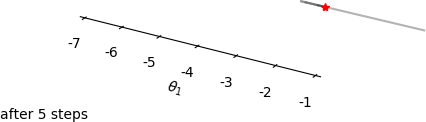
\includegraphics[width=200pt]{1d_5_trimmed.png} &
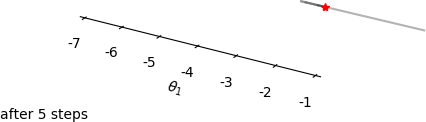
\includegraphics[width=.49\textwidth]{1d_5_trimmed.png} &
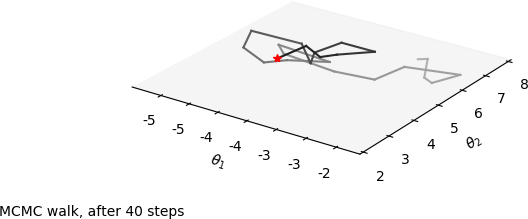
\includegraphics[width=.49\textwidth]{2d_40_trimmed.png} \\
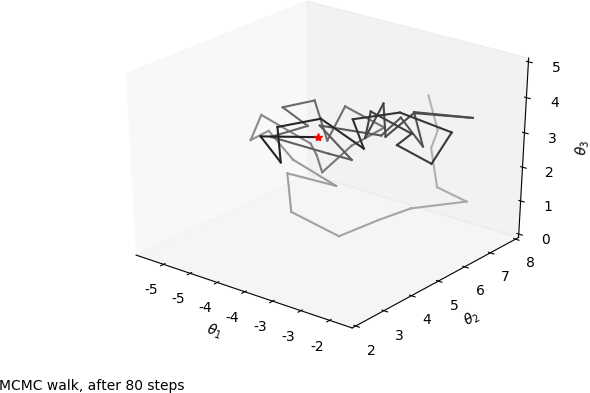
\includegraphics[width=.49\textwidth]{3d_80_trimmed.png} &
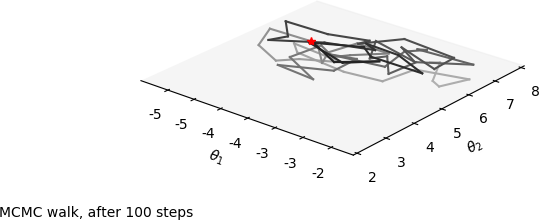
\includegraphics[width=.49\textwidth]{2d_100_trimmed.png} \\ 
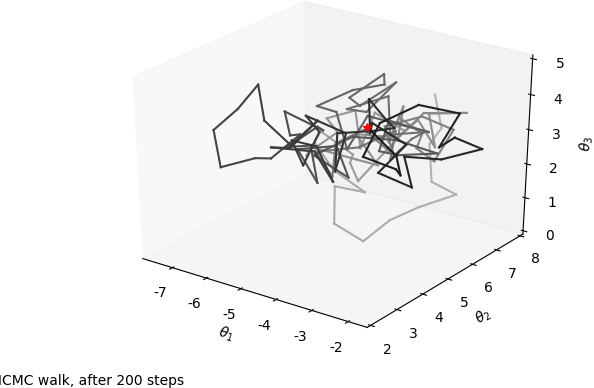
\includegraphics[width=.49\textwidth]{3d_200_trimmed.png} &
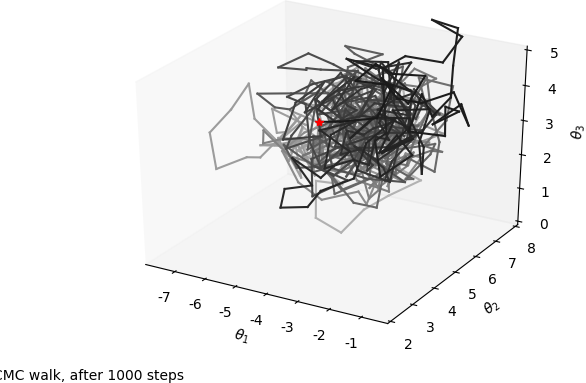
\includegraphics[width=.49\textwidth]{3d_1000_trimmed.png} \\
\end{tabular}
\caption{Model building, built into an MCMC walk: First start out with the
Standard Model, a zero-dimensional model. Try adding random first dimension,
say a scalar field (top
left). At a certain points, open up a random second dimension, e.g. a
fermionic field (top right),
then a third, e.g. another scalar (center left). Trimming might again reduce the number of
dimensions of your model (center right), but more dimensions might get added later
(bottom left), until the method converges (bottom right). Of course, this
simple idea that one field corresponds to one degree of freedom in the model
does not hold. For illustration only. }
\label{fig_models}
\end{center}
\end{figure}

Finally, Table~\ref{fractions} that shows the fraction 
of points within the signifcance isolines, and the expected fraction 
(by integrating the $\chi^2$ distributions with 3 dof),
for validation. Here is also a movie:\\
\href{http://smodels.hephy.at/walten/mcmc.webm}{http://smodels.hephy.at/walten/mcmc.webm}.

\begin{table}
\begin{tabular}{|c|c|c|}
\hline
	significance & fraction of points & expected fraction \\
\hline 
 1 $\sigma$  & 21\% & 20\% \\\hline
 2 $\sigma$  & 43\% & 42\% \\\hline
 3 $\sigma$  & 60\% & 61\% \\\hline
 4 $\sigma$  & 73\% & 74\% \\\hline
 5 $\sigma$  & 81\% & 83\% \\\hline
 6 $\sigma$  & 87\% & 89\% \\\hline
 7 $\sigma$  & 91\% & 93\% \\\hline
\end{tabular} 
\caption{Fraction of points within significance levels, for 4000 points. The
numbers pretty much match. }
\label{fractions}
\end{table}

\begin{figure}[h!t]
\begin{center}
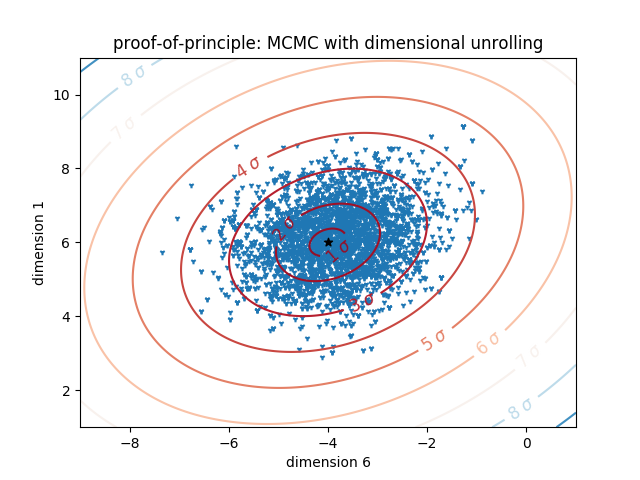
\includegraphics[width=300pt]{xy.png}
\caption{Final distribution of MCMC points, in the plane of the dimensions 1
and 6. The lines are the iso lines of the true significances. The black star
coressponds to the true center of the distribution. }
\label{fig_xy}
\end{center}
\end{figure}

\begin{figure}[h!t]
\begin{center}
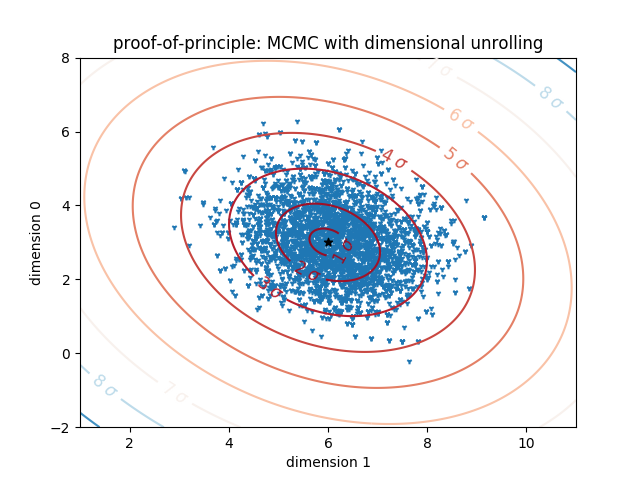
\includegraphics[width=300pt]{yz.png}
\caption{Final distribution of MCMC points, in the plane of the dimensions 6
and 0. The lines are the iso lines of the true significances.}
\label{fig_yz}
\end{center}
\end{figure}

\begin{figure}[h!t]
\begin{center}
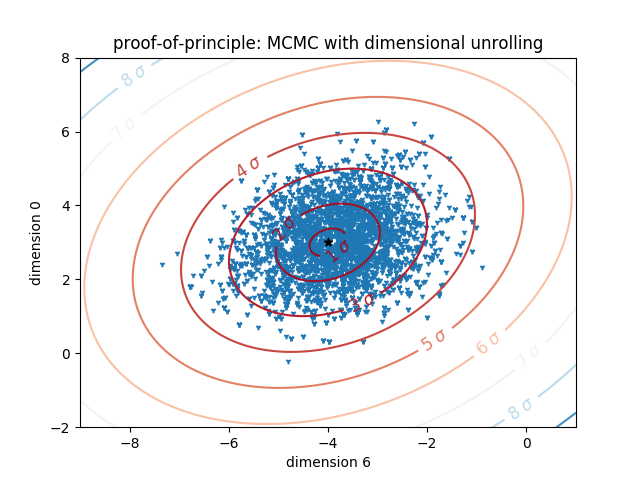
\includegraphics[width=300pt]{xz.png}
\caption{Final distribution of MCMC points, in the plane of the dimensions 1
and 0. The lines are the iso lines of the true significances.}
\label{fig_xz}
\end{center}
\end{figure}

\section{Prior and regularization}
In a Bayesian setting, the prior can be used to introduce regularization, e.g.
via:
\begin{equation}
  p \propto \frac{1}{n^{i}_{dims}}
\end{equation}

With $i=1,2,... $. Note that the prior can be improper.
\newpage

\section{On the space of all viable Lagrangians}

I dont yet understand what this could look like, i.e. what can and what cannot
be added to the Lagrangian to produce a consistent model? And how consistent
does it have to be? Does it have to be anomaly-free, renormalizable,
perturbative, unitary? Does the vacuum have to be stable? Etc, etc. 
But a few first ideas of what additional degrees of freedom we could start
with:

\subsection*{Dark photon}
\label{sec:photon}
We could add a $\gamma'$ that kinetically mixes with photons. Seems to be a
very simple thing to add, with only two degrees of freedom: the dark photon's
mass $m_{\gamma'}$ and its mixing angle $\kappa$.
\begin{figure}[h!t]
\begin{center}
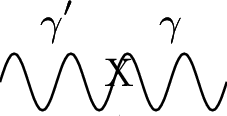
\includegraphics[width=60pt]{kinetic_mixing.png}
\caption{A dark photon that kinetically mixes with electromagnetic photons.}
\label{fig_darkphoton}
\end{center}
\end{figure}

\subsection*{Additional scalar}
\label{sec:scalar}
If we allow for one additional (real-valued or complex-valued) scalar whose
hypercharge (and color charge) is zero, then we also end up with a very simple
addition to the SM. The scalar acts as a dark matter candidate (is that true?)
with the Higgs being the portal to the SM. The (renormalizable) new terms in the Lagrangian
read:
\begin{equation}
 \Delta \mathcal{L} = \frac{1}{2} (\partial^{\mu} S) (\partial_{\mu} S) -
\frac{M^2}{2} S^{2} - \frac{g}{3} S^3 - g_{HS} (H^{\dagger} H) S -
\frac{\lambda_S}{4}S^4 - \frac{\lambda_{HS}}{2} (H^{\dagger} H) S^2
\end{equation}
which gives us immediately five more parameters (correct?).

\subsection*{Additional Higgs}
\label{sec:higgs}
Adding a second Higgs doublet, as in the two Higgs doublet models, seems also 
an option. Inert Higgs Doublet Models may also be interesting. 
When adding a second Higgs Doublet, one usually softly breaks $Z_2$ symmetry
(right?) which immediately leads to 8 degrees of freedom:
\begin{eqnarray}
 V = m_{11}^2 \Phi_1^\dagger \Phi_1 m_{22}^2 \Phi_2^\dagger \Phi_2 - m_{12}^2
\left( \Phi_1^\dagger \Phi_2 + \Phi_2^\dagger \Phi_1 \right) + \frac{1}{2}
\lambda_1 (\Phi_1^\dagger \Phi_1)^2  + \frac{1}{2} \lambda_2 (\Phi_2^\dagger
\Phi_2)^2 + \\ 
+ \lambda_3 (\Phi_1^\dagger \Phi_1) (\Phi_2^\dagger \Phi_2) +
\lambda_4 (\Phi_1^\dagger \Phi_2) (\Phi_2^\dagger \Phi_1) + \frac{1}{2}
\lambda_5 \left[ (\Phi_1^\dagger \Phi_2)^2 + (\Phi_2^\dagger \Phi_1)^2   \right]
\end{eqnarray}

\subsection*{Additional gauge group}
\label{sec:gauge}
Adding an additional gauge group like U(1)$_{B-L}$ seems more involved.

\section{First attempts based on SLHA files}
\label{sec:slha}
Learning directly Lagrangians is both from a technical and from a theoretical
point of view extremely challenging. A much easier task is learning models
that can be properly described with SLHA files, i.e. SUSY-inspired models.

\begin{figure}[h!t]
\begin{center}
\begin{tabular}{cc}
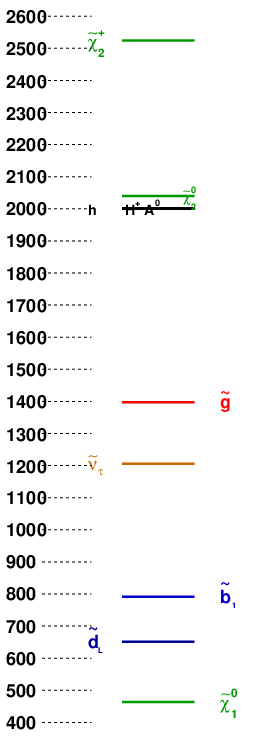
\includegraphics[width=.49\textwidth]{ruler.png} &
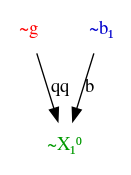
\includegraphics[width=.49\textwidth]{decays.png}
\end{tabular}
\caption{SLHA-based learned model, current hiscore ($Z=2.4$).}
\label{fig_hiscore}
\end{center}
\end{figure}

%\bibliography{algorithm}
%\bibliographystyle{abbrv} 

\end{document}
